\documentclass[12pt]{article}

% --------------------
% Packages
% --------------------
\usepackage[margin=1in]{geometry}
\usepackage{setspace}
\usepackage{graphicx}
\usepackage{amsmath, amssymb}
\usepackage{hyperref}
\usepackage{booktabs}
\usepackage{caption}
\usepackage{subcaption}
\usepackage{tikz}

% --------------------
% Formatting
% --------------------
\onehalfspacing
\setlength{\parindent}{0pt}
\setlength{\parskip}{1em}

% --------------------
% Title Information
% --------------------
\title{2-Layer MLP with Sigmoid Activation}
\author{Mahmudul Hasan}
\date{\today}

\begin{document}

\maketitle

% --------------------
% Abstract
% --------------------
% \begin{abstract}
% This is the abstract. Briefly summarize the purpose, methods, and conclusions of the article.
% \end{abstract}

% --------------------
% Main Sections
% --------------------
\section{Definitions}

\subsection{Multilayer Perceptron}
A Multilayer Perceptron (MLP) is a type of feedforward artificial neural network that consists of multiple layers of nodes. Each layer is fully connected to the next one, and the nodes in each layer apply a nonlinear activation function to their inputs. MLPs are commonly used for classification and regression tasks.

\subsection{Sigmoid Activation Function}
The sigmoid activation function is defined as:
\[\sigma(x) = \frac{1}{1 + e^{-x}} \]

The derivative of the sigmoid is given by:
\[\sigma'(x) = \frac{e^{-x}}{(1 + e^{-x})^2} = \sigma(x)\left(1 - \sigma(x)\right)\]

\section{2-Layer MLP}
\subsection{Network Architecture}

A 2-layer MLP with sigmoid activation consists of:
\begin{itemize}
    \item Input layer: $n$ nodes ($x_1, x_2, \ldots, x_n$)
    \item Hidden layer: $m$ nodes (pre-activation $z_1, z_2, \ldots, z_m$, post-activation $a_1, a_2, \ldots, a_m$) with sigmoid activation
    \item Output layer: 1 node (pre-activation $z_o$, output $o$) with sigmoid activation
\end{itemize}

\begin{figure}[h]
    \centering
    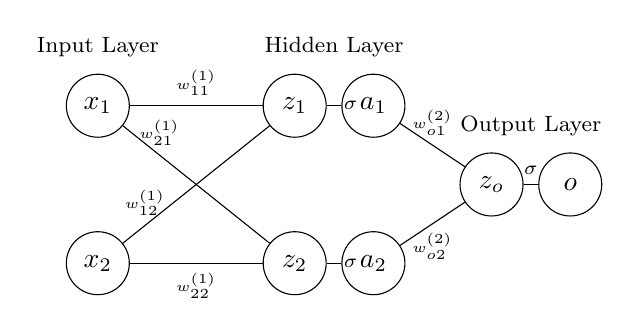
\begin{tikzpicture}[node distance=2cm]
        % Input nodes
            \node[circle, draw, minimum size=0.8cm] (x1) at (0, 2) {$x_1$};
            \node[circle, draw, minimum size=0.8cm] (x2) at (0, 0) {$x_2$};
            
            % Hidden layer nodes (pre-activation)
            \node[circle, draw, minimum size=0.8cm] (z1) at (2.5, 2) {$z_1$};
            \node[circle, draw, minimum size=0.8cm] (z2) at (2.5, 0) {$z_2$};
            
            % Hidden layer nodes (post-activation)
            \node[circle, draw, minimum size=0.8cm] (a1) at (3.5, 2) {$a_1$};
            \node[circle, draw, minimum size=0.8cm] (a2) at (3.5, 0) {$a_2$};
            
            % Output node (pre-activation and output)
            \node[circle, draw, minimum size=0.8cm] (zo) at (5, 1) {$z_o$};
            \node[circle, draw, minimum size=0.8cm] (out) at (6, 1) {$o$};
            
            % Connections: input to hidden (pre-activation)
            \draw (x1) -- (z1) node[midway, above, font=\tiny] {$w_{11}^{(1)}$};
            \draw (x1) -- (z2) node[pos=0.25, above, font=\tiny] {$w_{21}^{(1)}$};
            \draw (x2) -- (z1) node[pos=0.15, above, font=\tiny] {$w_{12}^{(1)}$};
            \draw (x2) -- (z2) node[midway, below, font=\tiny] {$w_{22}^{(1)}$};
            
            % Activation function (hidden layer)
            \draw (z1) -- (a1) node[midway, right, font=\scriptsize] {$\sigma$};
            \draw (z2) -- (a2) node[midway, right, font=\scriptsize] {$\sigma$};
            
            % Connections: hidden (post-activation) to output (pre-activation)
            \draw (a1) -- (zo) node[midway, above, font=\tiny] {$w_{o1}^{(2)}$};
            \draw (a2) -- (zo) node[midway, below, font=\tiny] {$w_{o2}^{(2)}$};
            
            % Activation function (output layer)
            \draw (zo) -- (out) node[midway, above, font=\scriptsize] {$\sigma$};
            
            % Labels
            \node[above, font=\footnotesize] at (0, 2.5) {Input Layer};
            \node[above, font=\footnotesize] at (3, 2.5) {Hidden Layer};
            \node[above, font=\footnotesize] at (5.5, 1.5) {Output Layer};
    \end{tikzpicture}
    \caption{Architecture of a 2-layer MLP (shown for $n=2$, $m=2$ example)}
\end{figure}

Here, $w_{ji}^{(1)}$ represents the weight from the $i$-th input node to the $j$-th hidden node (pre-activation), and $w_{oj}^{(2)}$ represents the weight from the $j$-th hidden node (post-activation) to the output pre-activation node. The sigmoid activation function $\sigma$ is applied after each layer.

\subsection{Forward Pass}

In general, the forward pass for each hidden node $j$ (where $j = 1, 2, \ldots, m$) is:
\begin{align*}
z_j &= \sum_{i=1}^{n} w_{ji}^{(1)} x_i + b_j^{(1)} \\
a_j &= \sigma(z_j)
\end{align*}

And for the single output node:
\begin{align*}
z_o &= \sum_{j=1}^{m} w_{oj}^{(2)} a_j + b_o^{(2)} \\
o &= \sigma(z_o)
\end{align*}

In general matrix form, let the input vector be $\mathbf{x} = [x_1 \space\space x_2 \space\space \ldots \space\space x_n]^T \in \mathbb{R}^{n \times 1}$ (column vector). The weights for the hidden layer are represented as a matrix $\mathbf{W}^{(1)} \in \mathbb{R}^{m \times n}$, where row $j$ contains all weights going to hidden node $j$. With our indexing convention where $w_{ji}^{(1)}$ connects input $i$ to hidden $j$, the weight matrix has elements $[\mathbf{W}^{(1)}]_{ji} = w_{ji}^{(1)}$. The pre-activation output of the hidden layer can be calculated as:

\[ \mathbf{z}^{(1)} = \mathbf{W}^{(1)} \mathbf{x} + \mathbf{b}^{(1)} \]

where $\mathbf{b}^{(1)} \in \mathbb{R}^m$ is the bias vector for the hidden layer. The post-activation output is:

\[ \mathbf{a}^{(1)} = \sigma\left(\mathbf{z}^{(1)}\right) \]

The pre-activation output of the network can then be calculated as:

\[ z_o = \mathbf{w}^{(2)} \mathbf{a}^{(1)} + b_o^{(2)} \]

where $\mathbf{w}^{(2)} = [w_{o1}^{(2)}, w_{o2}^{(2)}, \ldots, w_{om}^{(2)}]^T \in \mathbb{R}^m$ is the weight vector for the output layer and $b_o^{(2)}$ is the bias scalar for the single output node. Finally, the output is:

\[ o = \sigma\left(z_o\right) \]

\subsection{Loss Function}

The loss is calculated over a batch of $N$ training examples using Mean Squared Error (MSE):

\[ \mathcal{L} = \frac{1}{N} \sum_{k=1}^{N} (y^{(k)} - o^{(k)})^2 \]

where $y^{(k)}$ is the true label and $o^{(k)}$ is the predicted output for the $k$-th training example in the batch. The superscript $(k)$ denotes the sample index to distinguish it from node indices.

\subsection{Gradients of the Loss Function}
To update the weights during training, we need to compute the gradients of the loss function with respect to the weights. Using backpropagation, we can derive the gradients as follows:

\textbf{Gradient for output layer weights:}

For each weight connecting hidden node $j$ (where $j = 1, 2, \ldots, m$) to the output, we apply the chain rule:
\begin{align*}
\frac{\partial \mathcal{L}}{\partial w_{oj}^{(2)}} &= \frac{\partial \mathcal{L}}{\partial o} \cdot \frac{\partial o}{\partial z_o} \cdot \frac{\partial z_o}{\partial w_{oj}^{(2)}} \\
&= \frac{2}{N}(o - y) \cdot \sigma'(z_o) \cdot a_j
\end{align*}

\textbf{Gradient for output layer bias:}
\begin{align*}
\frac{\partial \mathcal{L}}{\partial b_o^{(2)}} &= \frac{\partial \mathcal{L}}{\partial o} \cdot \frac{\partial o}{\partial z_o} \cdot \frac{\partial z_o}{\partial b_o^{(2)}} \\
&= \frac{2}{N}(o - y) \cdot \sigma'(z_o)
\end{align*}

\textbf{Gradient for hidden layer weights:}

For the hidden layer, we need to backpropagate through the output layer. Since there is only one output node, the gradient for each weight $w_{ji}^{(1)}$ (where $i = 1, 2, \ldots, n$ and $j = 1, 2, \ldots, m$) is:
\begin{align*}
\frac{\partial \mathcal{L}}{\partial w_{ji}^{(1)}}
&= \frac{\partial \mathcal{L}}{\partial o} \cdot \frac{\partial o}{\partial z_o} \cdot \frac{\partial z_o}{\partial a_j} \cdot \frac{\partial a_j}{\partial z_j} \cdot \frac{\partial z_j}{\partial w_{ji}^{(1)}} \\
&= \frac{2}{N}(o - y) \cdot \sigma'(z_o) \cdot w_{oj}^{(2)} \cdot \sigma'(z_j) \cdot x_i
\end{align*}

where $\frac{\partial z_o}{\partial a_j} = w_{oj}^{(2)}$ (from $z_o = \sum_{j=1}^m w_{oj}^{(2)} a_j + b_o^{(2)}$) and $\frac{\partial z_j}{\partial w_{ji}^{(1)}} = x_i$ (from $z_j = \sum_{i=1}^n w_{ji}^{(1)} x_i + b_j^{(1)}$).

\textbf{Gradient for hidden layer biases:}

For each hidden layer bias $b_j^{(1)}$ (where $j = 1, 2, \ldots, m$):
\begin{align*}
\frac{\partial \mathcal{L}}{\partial b_j^{(1)}} &= \frac{\partial \mathcal{L}}{\partial o} \cdot \frac{\partial o}{\partial z_o} \cdot \frac{\partial z_o}{\partial a_j} \cdot \frac{\partial a_j}{\partial z_j} \cdot \frac{\partial z_j}{\partial b_j^{(1)}} \\
&= \frac{2}{N}(o - y) \cdot \sigma'(z_o) \cdot w_{oj}^{(2)} \cdot \sigma'(z_j)
\end{align*}

% \section{Methodology}
% Describe methods, models, or experimental setup.

% \section{Results}
% Present results, tables, and figures.

% \section{Discussion}
% Interpret results and discuss implications.

% \section{Conclusion}
% Summarize findings and suggest future work.

% % --------------------
% % Acknowledgments
% % --------------------
% \section*{Acknowledgments}
% Optional acknowledgments go here.

% % --------------------
% % References
% % --------------------
% \bibliographystyle{plain}
% \bibliography{references}

\end{document}
